\section{Durchführung} \label{sec:Durchführung}

\subsection{Aufbau der Messapparatur}

    \begin{figure}
      \centering
      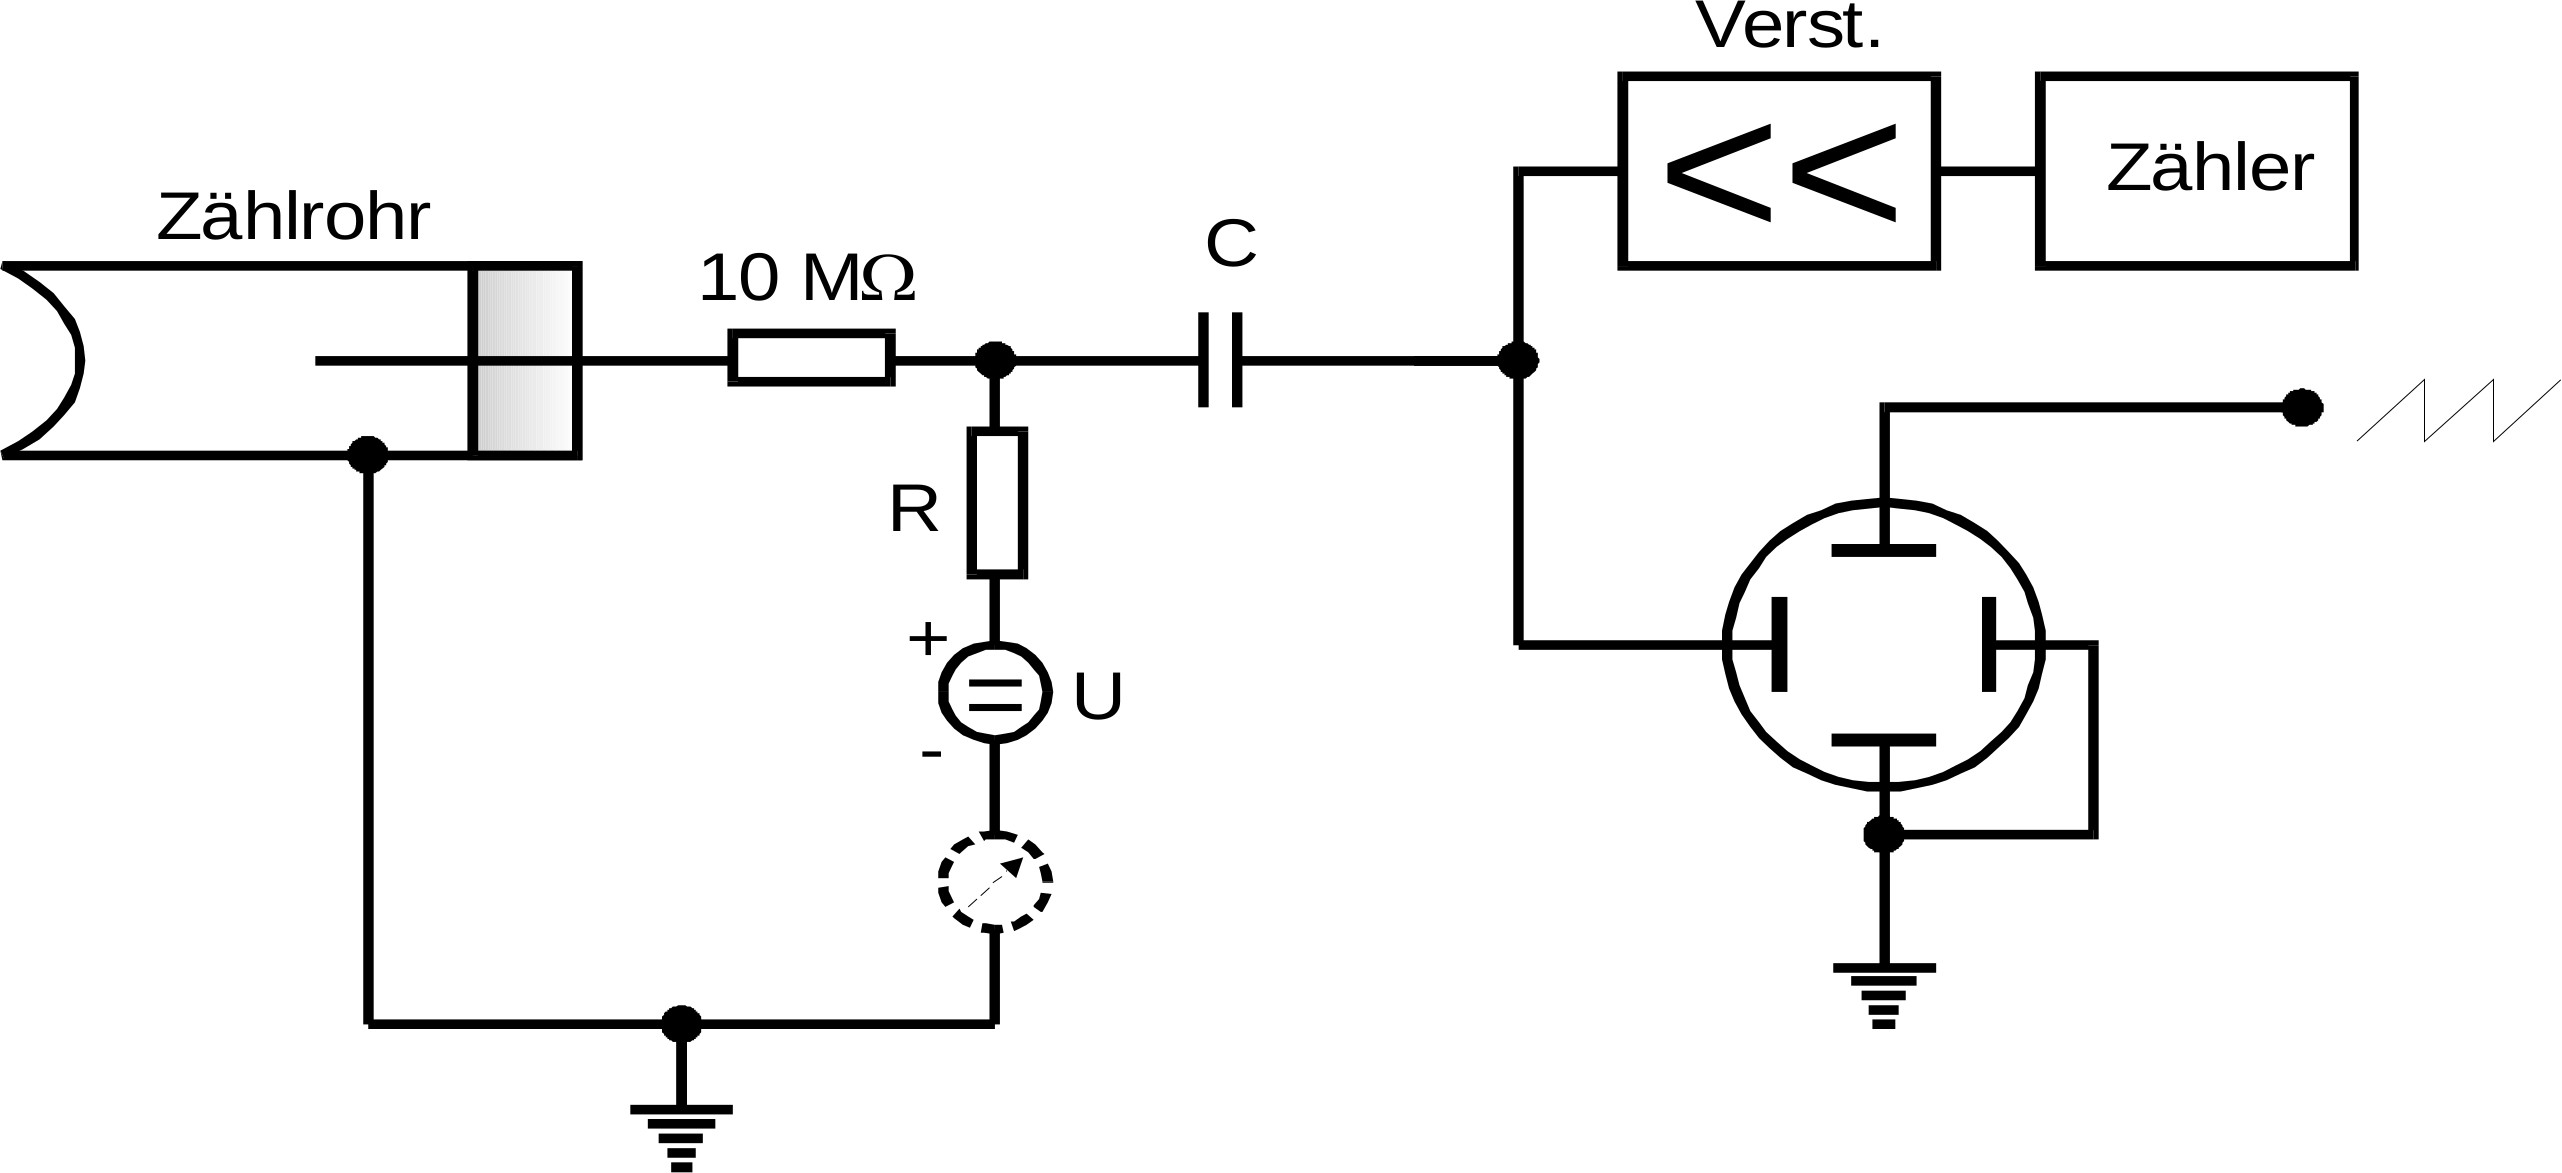
\includegraphics[width=0.75\textwidth]{content/img/V703_Abb5.jpg}
      \caption{Skizze der Messapparatur \cite{versuchsanleitung}.}
      \label{fig:abb5}
    \end{figure}

    In \autoref{sec:Theorie} der theoretischen Grundlagen wurde der Aufbau des Geiger-Müller-Zählrohrs erklärt.
    In \autoref{fig:abb5} ist nun der Aufbau einer Messapparatur gezeigt,
    mit der weitere Untersuchungen der gemessenen Impulse durchgeführt werden könnnen. \\
    Die an der Anode im Inneren des Zählrohrs auftreffenden Elektronen mit der gesammelten
    Ladung $Q$ fließen durch den Draht über einen Widerstand $R$ ab.
    Infolge dessen wird ein Spannungsimpuls erzeugt,
    der über einen Kondensator ausgekoppelt und in einem Zählgerät gemessen wird.

\subsection{Geiger-Müller-Zählrohr Charakteristik} \label{sec:charaktbestimmen}

    Um die Zählrate zu messen, wird eine $\ce{^204Tl}$-Quelle vor das Eingangsfenster
    des Geiger-Müller-Zählrohrs gestellt. Die maximale Impulsrate der auftreffenden
    Elektronen sollte bei maximal $\SI{100}{\per\second}$ liegen.
    %um Korrekturen bei der Totzeit zu vermeiden. %????
    Für die Messung wird die anliegende Spannung $U$ in Schritten von $\symup{\Delta}U = \SI{10}{\volt}$
    über eine Zeit von $t = \SI{60}{\second}$ erhöht,
    wobei das Maximum des Zählrohrs bei $\SI{700}{\volt}$ liegt, um eine Dauerentladung
    zu vermeiden.
    %Größenordnung des Zählrohrs?
    Zusätzlich wird der Zählrohrstrom $I$ gemessen, welcher durch die freien Elektronen
    entsteht, mit einer Ablesegenauigkeit von $\symup{\Delta}I = \SI{0.05}{\micro\ampere}$.

 \subsection{Zählrohrstrom}

    Um die Teilchenzahl $Z$ zu bestimmen, kann der bei der Erstellung der Zählrohr-Charakteristik
    gemessene Zählrohrstrom $I$ verwendet werden.
    Es gilt \autoref{eqn:Teilchenzahl}.

\subsection{Totzeit und Nachentladung}

    Die Totzeit kann bei hoher Strahlungsintensität auf einem Oszillographen abgelesen werden,
    weshalb die $\ce{^204Tl}$-Quelle näher an die Zählröhre gestellt wird.
    Zusätzlich wird über eine Zeit von $t = \SI{120}{\second}$ gemessen. \\
    Zur Bestimmung der Totzeit wird die Zwei-Quellen-Methode verwendet.
    Diese funktioniert so, dass zuerst die Zählrate $N_1$ eines ersten Präparates im
    Geiger-Müller-Zählrohr gemessen wird.
    Dann wird ein zweites Präparat hinzugefügt, ohne das erste zu entfernen,
    und misst die Zählrate $N_{1+2}$.
    Anschließend wird das erste Präparat entfernt und die Zählrate $N_2$ des zweiten
    gemessen.
    % Die Totzeit kann mit Gleichung \eqref{eqn:totzeit} bestimmt werden und ist auf
    Die Totzeit kann mit \autoref{eqn:totzeit} bestimmt werden und ist auf
    einem Oszillographen sichtbar.\\
    \\
    Für die Messung der Nachentladung wird die Strahlungsintensität verringert.
    Die Ablenkgeschwindigkeit des Kathodenstrahls liegt bei $\SI{50}{\micro\second\per\centi\meter}$.
    Die verwendete Spannung $U$ liegt zu Anfang bei $\SI{350}{\volt}$ und wird zur Messung auf
    $\SI{700}{\volt}$ geregelt. Es wird der zeitliche Abstand zwischen Primär- und Nachentladungsimpuls
    gemessen.

%\subsection{Zählrohrstrom}

    %Um die Teilchenzahl $Z$ zu bestimmen, kann der bei der Erstellung der Zählrohr-Charakteristik
    %gemessene Zählrohrstrom $I$ verwendet werden. Es gilt die \autoref{eqn:Teilchenzahl}.







    %Zur Messung der Zählrate wird eine $\beta$-Quelle vor das Geiger-Müller-Zählrohr gestellt.
    %Die Spannung $U$, die am Zählrohr anliegt, muss unter $\SI{700}{\volt}$ liegen,
    %damit es nicht zu einer Dauerentladung kommt.
    %Die maximale Impulsrate der auftreffenden Elektronen sollte bei maximal $\SI{100}{\frac{1}{\second}}$
    %liegen, um Korrekturen bei der Totzeit zu vermeiden.
    %Die Totzeit kann bei hoher Strahlungsintensität auf einem Oszillographen abgelesen werden,
    %sofern die Ablenkgeschwindigkeit des Kathodenstrahls im elektrischen Feld bekannt ist.
    %Bei einer geringen Strahlungsintensität kann auf einem Oszillographen die Nachentladung sichtbar
    %gemacht werden. Für diese Messung liegt die Ablenkgeschwindigkeit bei $\SI{50}{\micro\second\per\centi\meter}$.
    %Die verwendete Spannung $U$ liegt zu Anfang bei $\SI{350}{\volt}$ und wird zur Messung auf
    %$\SI{700}{\volt}$ geregelt. Es wird der zeitliche Abstand zwischen Primär- und Nachentladungsimpuls
    %gemessen.
